\documentclass[11pt, a4paper]{article}
\usepackage{times}
\usepackage{latexsym}
\usepackage{graphicx}
\usepackage{url}
\usepackage{breakcites}

\title{Hyperpartisan News Detection}

\author{Rebekah Cramerus \\
  MSc Cognitive Systems \\
  University of Potsdam \\
  {\tt {\small rebekah.cramerus@fulbrightmail.org}} \\}

\date{}

\begin{document}
\maketitle
\begin{abstract}
This paper reports on my Individual Module for the Masters in Cognitive Systems at the University of Potsdam. The project question was taken from SemEval 2019 Task 4 (Hyperpartisan News Detection), the shared task which I also participated in. The goal was binary classification of news articles into the categories of ``biased" or ``unbiased". The primary problem encountered during the course of the project was the noise in the provided datasets, and the models' subsequent tendency to learn publisher-specific traits instead of general bias. Various approaches were taken to try and combat this issue, using both handcrafted linguistic features and neural networks, two of which were submitted to SemEval for inclusion on the leaderboard. Generally, though some progress was made, the different approaches were not able to overcome the inherent noise in the data.
\end{abstract}

\section{Introduction}

With the proliferation of online news agencies after the rise of the Internet, access to information about what is going on in the world has never been more widespread. How that information is presented, however, can have a large influence on what conclusions the reader draws from it. Being able to automatically identify hyperpartisanship (bias or adherence to one party or faction over others) in a news article would help individuals in their news consumption and potentially result in a better-informed population. 

As suggested, the challenge approached in this paper is that of hyperpartisan news detection: a binary classification problem (biased or unbiased) with news articles as data. This task can be considered as related to stance detection and in general, sentiment analysis. The challenge was originally organized as Task 4 for SemEval 2019 \cite{potthast:2018} \cite{kiesel:2019}. 

I took various approaches to the task. Among them were approaches that focused on handcrafted linguistic features: a basic unigram (bag-of-words) model and one that included such features as dependency tags, parts of speech and emotive words. Beyond those approaches, I developed models using deep learning to tackle the problem in a different manner. I used dataset-trained word embeddings and a type of neural network called Long Short Term Memory (LSTM) networks, as well as vectorization of the whole document (doc2vec) paired with a feedforward neural network. In order to reduce the noise in the dataset, a voting system was introduced to pare down the training dataset to those examples which were confidently biased. Models were trained on different subsets of publishers and only those examples which were correctly labeled as biased by all voters were kept for a cleaner dataset.

Generally, the models showed higher recall than precision, and hovered around 60\% accuracy on datasets which included different publishers than those they were trained on. However, the neural networks were often able to perform well on holdout test sets from the same publishers.

In this paper, Section 2 provides an overview of previous literature in the topic of bias detection and related problems. Section 3 includes an introduction of the provided dataset and a description of preprocessing techniques used for our approach. Section 4 describes each aforementioned experiment for the task. Section 5 presents results of all approaches and Section 6 delves into analysis, presenting potential reasons why the models did not perform very well. Finally, Section 7 elaborates on what could have been done and what could be done in the future for better work.

\subsection{SemEval Task 4}

The International Workshop on Semantic Evaluation takes place each year and focuses on evaluating semantic analysis systems through providing a number of shared tasks for the public to participate in. This project was structured according to Task 4: Hyperpartisan News Detection among 2019's set of tasks.

Training and validation datasets were provided to participants, and final submissions were submitted through TIRA, with the test datasets hidden, through the use of a provided virtual machine \cite{potthast:2019}.

Our team name was Kit Kittredge, after the American Girl doll whose character wanted to become a reporter.

\section{Previous Work}

Before starting work on the task itself, I conducted a literature review into past research on bias detection, bias labeling, and related topics such as sentiment analysis, subjectivity, stance detection and opinion mining.

Distinguishing these topics from one another can be a challenge in and of itself. Yano et al (2010) conducted an empirical study of linguistic indicators of political bias, and noted that whereas \textit{subjectivty} in NLP is an author communicating their own thoughts, \textit{bias} is a ``tendency or preference towards a particular persective, ideology or result": a predefined prediliction shared by a group of people rather than an individual opinion \cite{yano2010shedding}. However, ways to approach bias and subjectivity problems often have significant overlap.

Recasens et al (2013) reveals two types of bias: epistemological and framing. The former focuses on assumptions or presupposed propositions in a text, and can be seen bidirectionally, when a fact generally accepted as true has doubt cast upon it, or when a generally uncertain fact is stated with certainty \cite{recasens2013linguistic}. Framing bias, on the other hand, describes perspective-specific words or phrases, meant to show a topic in a particular way.

Hyperpartisan detection in the context of this paper necessitates detecting, in general, if a document is biased or not, not in which political direction the bias leans. Most previous research, however, focuses on right vs. left (usually in an American context) identification on already biased sentences, with a lack of neutral or unbiased text. Furthermore, many approaches were based upon data compiled and labeled at the sentence level \cite{conrad2012recognizing} \cite{somasundaran2010recognizing}. A lack of clearly labeled and clean datasets means that many papers conducted their own data gathering processes using crowdsourcing software. Generally, the literature focuses on gathering well-labeled data, unigram-focused approaches, and in increasingly more cases, machine learning models with more complex linguistic features to capture syntactic relations.

\subsection{N-grams} \label{ngrams}

Most research in the area considers n-grams in one way or another: for a bag-of-words baseline, through specially crafted vocabularies (see \ref{premade-lexicons}), or in taking the whole vocabulary as count or TF-IDF vectors as additional features. It seems generally agreed upon that lexical variation is an important reflector of ideological views; Lin et al (2008) focused on developing statistical models for distributions of words according to topic and ideological perspective \cite{lin2008jointtopic}.

Wiebe et al (2004) makes an interesting and important observation: hapax legomena, or the set of words which appear just once in a corpus, have a high correlation with subjective language; apparently, people are more creative when they write with strong feeling \cite{wiebe2004learning}. In fact, they find that many good clues of subjectivity occur with low frequency, and this correlation naturally becomes stronger with a larger corpus.

Certain kinds of words are frequently mentioned as high indicators of bias. Hedges (``may", ``possibly") reduce an author's dedication to a statement, assertive verbs (``stated" versus ``claimed") give a implicit claim on the truth of a statement as do factive verbs (``reveal" versus ``indicate"), entailments carry other implications (``murder" versus ``kill") \cite{recasens2013linguistic}.

\subsection{Premade Lexicons} \label{premade-lexicons}

Many projects have focused on compiling lists of words that contribute to subjectivity, polarity, emotion or bias in some way, and a handful of these lexicons were used in this paper.

One major set of vocabularies was created by Wilson et al (2005): the MPQA Lexicons for subjectivity, polarity effect and arguing. \cite{wilson2005recognizing}. After extraction of prior-labeled polarity clues, labeling is done with a strict rule-based system which looks at modifiers, negators and adverbs to give the final classification of the phrase polarity. The authors noted that often, subjectivity clues would appear in contexts that overall did not share their polarity, indicating that context is crucial. This set of lexicons is often referenced in other papers, to varying results: Lin et al (2011) took a weakly-supervised generative model approach to sentence-level subjectivity detection, using the MPQA strongly subjective clues as their words of known polarity \cite{lin2011sentence}. Importantly, they argue that to obtain good results it is necessary to filter \textit{out} neutral words, as their dominance in terms of frequency (there being more neutral words in a text than subjective ones) biases a model towards classifying a text as objective. 

Like in Wilson et al (2005), many approaches used a ``seed" set of manually labeled words to extrapolate to a larger vocabulary using a corpus. Godbole et al (2007) focused on domain-specific lexicons for sentiment analysis (general, health, crime, sports, business, politics and media), each category having positive and negative vocabularies, grown from the seed wordsets using recursion and path-following techniques \cite{godbole2007largescale}.

Wiebe et al (2004) developed a method for automatically identifying and collecting collocational clues, to extract a vocabulary of subjective words specific to the domain of a given corpus \cite{wiebe2004learning}. Noting that the data of a corpus of documents is inherently noisy, as opinion pieces will contain non-subjective sentences and neutral texts will similarly have some subjective parts, they start with a labeled seed set of words and use distributional similarity to expand the vocabulary. The authors find good results on classifying subjective texts with their collected vocabulary, finding an accuracy of 94\% on a large test set.

While most of the previously described literature focuses on general subjectivity detection instead of bias, some work has been done on partisanship. Gentzkow and Shapiro (2010) aimed to rate ideological leaning of newspapers as a whole, based on frequency of appearance of short partisan collocations \cite{gentzkow2010whatdrives}. Some examples given from their phrase selection process were ``death tax", and ``war on terror" versus ``war in Iraq".

\subsection{Linguistic Features}

There are a number of common features, meant to capture various aspects of syntactic structure, which are used in machine learning approaches to questions of bias, subjectivity and general sentiment.

Part of speech tags are naturally among the most common; some approaches also use as features for each word the tags of the words in their surrounding context \cite{recasens2013linguistic}. Research shows a high correlation between adjectives and sentence subjectivity \cite{pang2008opinion}.

Dependency tree syntax features can also help with modality identification (``must", ``should", ``ought"), an important marker to find opinions or assertions, or passive voice, used to shift blame (``Mistakes were made.") \cite{somasundaran2010recognizing} \cite{pang2008opinion}. Greene and Resnik (2009) look at syntactic framing to identify sentiment. They recognize that certain properties of particular verbs, as discussed in \ref{ngrams}, are important features in determining sentiment, but note that often these properties are not directly observable. Hence they propose using syntactic relations as proxies to find the semantic aspects of the verbs \cite{greene2009syntactic}. However, there have been mixed results in evaluating the usefulness of dependency features with these tasks. Both Somasundaran and Wiebe (2010) and Anand et al (2011) described unigram baselines either outperforming or being close to sentiment models with dependency features \cite{somasundaran2010recognizing} \cite{anand2011classifying}.

Traditional readability features such as average document length, sentence length and word length are also commonly included as features \cite{leban2014news}.

\subsection{Topic Modeling}

Identifying what a document is about can go a long way in labeling the bias of the piece, given that ideological perspectives often come with defined and shared views on a variety of topics. Lin et al (2008) argues that modeling ideological discourse cannot be done without taking topic into account: words should be evaluated both on how they are related to the text's topic and on how the word relates to a particular ideological perspective \cite{lin2008jointtopic}. Latent Dirichlet Allocation (LDA) statistical models are a common choice for topic modeling. Nguyen et al (2013) uses supervised hierarchical LDA models to experiment with agenda setting and framing (portraying a topic in a certain way using language) to define how different language users approach different topics \cite{nguyen2013lexical}. Doumit and Minai (2012) use LDAs to explore how bias is embedded into the semantic description (the ``very fabric") of news \cite{doumit2012online}. Presumably, an ideal approach to bias detection would take not only lexical and syntactic, but semantic aspects in its features.

\subsection{Discourse Structure}

I found only a few papers that attempted to address discourse structure in their approaches. However, for bias detection and for sentiment analysis in general, discourse structure is certainly relevant; Pang and Lee (2008) note that position matters for sentiments in a document, and the \textit{global} sentiment for a piece can be modeled as a trajectory of \textit{local} sentiment \cite{pang2008opinion}. Conrad et al (2012) use 15 binary features for different discourse relations in their approach, suggesting that, for example, the presence of concessions could indicate a more neutral or non-biased perspective in terms of political partisanship \cite{conrad2012recognizing}.

Interestingly, Anand et al (2011) looked to identify agreement and disagreement relations in online forum posts \cite{anand2011classifying}. They trained a classifier using post metadata, unigrams and bigrams, dependency tags, part-of-speech tags, MPQA opinion words, context features and certain punctuation appearances, but, as previously mentioned, found that the dependency features had an overall lack of impact and it was difficult in all cases to beat a simple unigram baseline.

\subsection{Neural Networks}

Deep learning approaches have grown more common in recent years; their potential to capture various aspects of language and their interaction makes them a powerful tool.

Considering that most existing approaches, as delineated in the previous subsections, have focused on lists of words or n-grams, Iyyer et al chose to model the compositional aspects of language using neural networks \cite{iyyer2014political}. They note that within a document, bias may be found in a specific locale rather than over the entire piece. Therefore, it may be hard to find using traditional approaches of looking at all words. The authors focus on identifying bias at the sentence level: the problem was not, as such, the labeling of biased or unbiased, but left or right (no neutral), and where the bias is located. 

\begin{figure}
\centering
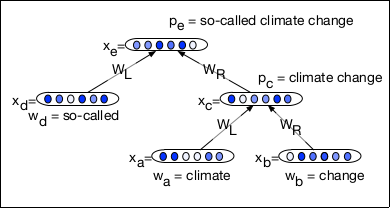
\includegraphics[width=200pt]{iyyer2014political.png}
\caption{Depiction of the percolation of phrase vectors from the original words from Iyyer et al (2014).}
\label{fig:iyyer2014tree}
\end{figure}

First, they developed their own dataset on political ideology annotated at the phrase level using crowdsourcing and active learning; the result was a dataset with 3,412 sentences containing 13,640 annotated nodes. They vectorized the texts using a pre-trained Google News word2vec embedding, and feature vectors were created for each phrase in the syntax tree for a sentence by percolating up from the leaves (Figure \ref{fig:iyyer2014tree}) \cite{mikolov2013word2vec}. A recursive neural network (RNN) was trained on this data and achieved about 70\% accuracy. Iyyer et al conclude that RNNs in this context are able to model the structural aspects of bias in language; an example provided is the bias for the phrase ``free market ideology" changing once it combines with a higher level phrase, ``made worse by".

Bellows (2018) provides an overview of the current work in the field of bias recognition \cite{bellows2018classify}. They conducted experiments using different common word embeddings (word2vec, GloVe, fasttext) and machine learning models (support vector machines, multilayer perceptrons, convolutional neural networks, and recursive neural networks), with results showing no front-runner among either group. On their sentence-level dataset, all models achieved between 74\% and 78\% accuracy.

\subsection{Problems with Datasets}

Relevantly, much of the literature documented issues with noise, vague labels, and other problems in corpora, particularly at the document level. Various approaches focused on a certain domain or set of domains, but often domain-specific models can have transfer problems, as what makes a text in one domain biased or subjective in a certain way may differ from a different area. Defining bias as a whole, therefore, may require a different or unique approach from domain-specific bias.

As previously mentioned, generally biased documents may have unbiased sentences, just as unbiased documents may contain biased sentences (perhaps as quotations, but also just as part of the main text). These non-matching segments can lead to document misclassification; to take these into account is a difficult task, as the overall sentiment for a text may be a function of the labels at the sentence level \cite{pang2008opinion}.

Sim et al (2013) explore the speeches of political candidates as ``sequences of cues interspersed with lags", defining documents as mostly irrelevant filler texts between ideological cues which on their own define the positioning of a document. They note that while cues which are closer to be one another tend to be of the same ideology, using a hidden Markov model (HMM) where states correspond to ideologies and emissions are a cue and the lag after it to model the progression of ideology in a speech \cite{sim2013measuring}. Importantly, they note systematic issues with using the candidates' names as cue terms. 

Crowdsourcing labels for datasets (often using Amazon's Mechanical Turk) reveals that the task of labeling bias can be difficult even for humans. Recasens et al (2013) note this particularly for their task of identifying a bias-inducing word given a biased sentence \cite{recasens2013linguistic}. Attempting human annotation on their dataset, composed of real instances of Wikipedia edits to remove bias from articles, produced only 30\% accuracy, although they acknowledge that this could suggest problems with the dataset and not the humans. Alternatively, it could suggest that people are predisposed to make bias judgments of other texts according to their own opinions, which differ greatly among a population.

Maynard et al (2012) use a particular dataset which brings with it a unique set of challenges: tweets \cite{maynard2012automatic}. With their shorter length, tweets do not contain a lot of context, and often require a world knowledge database to understand. Parsers struggle with tweets, and it is common to take ``extralinguistic" features from them such as hashtags and emoticons. The prevalence of irony and sarcasm also poses a challenge. Maynard et al achieve results which are high in precision at the expense of recall, and suggest that a succesful approach would focus on identifying ``powerful indicator words" which carry a strong political bias.

Finally, Leban et al (2014) tackle a different question than other papers, focusing on differences between specific publishers instead of more general differences between types of news sources or addressing bias itself \cite{leban2014news}. They found measurable differences between publishers in such features as part of speech tags and in particular article length.

\section{Data}

The datasets used in this project were those provided by SemEval for the shared Task 4.

\subsection{Usable Datasets}

A training dataset of 600,000 articles and a validation dataset of 150,000 articles were released to participants. Both sets contain 50\% unbiased and 50\% biased articles, and of the latter, half are left-biased and the other half right-biased (in terms of their placement on the political spectrum). Importantly, these articles were all labeled with the overall bias of their publisher, which was obtained by MediaBiasFactCheck.com and BuzzFeed. The set of publishers whose articles appear in the training set has no overlap with the publishers of the validation set, and neither has any overlap with the publishers whose articles appear in the inaccessible test set.

We consider the labels of these datasets to be noisy: though publishers may have an overall bias, it is likely that most biased news agencies do not publish only biased articles, just as most unbiased news agencies may occasionally publish a biased piece.

Also relevant is a third released dataset referred to in this paper as the \textit{byarticle} dataset. Unlike the other datasets, this one contains articles which were labeled individually through crowdsourcing. It is small, at 645 articles, and unbalanced, at 63\% unbiased and 37\% hyperpartisan.

\subsection{Hidden Datasets}

Finally, there are the hidden test datasets. One of the two test datasets was labeled individually by article, referred to in this paper as the \textit{byarticle-test} dataset, including 638 articles with no publisher overlap with any of the given corpora. The other, like the training and validation sets, was labeled overall by publisher, here referred to as the \textit{bypublisher-test} dataset, with a total of 4000 articles, also including no publisher overlap with other datasets.

These datasets are only accessed after using TIRA and then requesting that the results be revealed by the task organizers. The datasets themselves cannot be accessed or studied. Since we were allowed two software submissions, I submitted the bag-of-words model and the LSTM trained on the dataset reduced by the voting system, and as such only have results for the test datasets for those two systems. Otherwise, the byarticle dataset was used as my test dataset for the other approaches.

\subsection{Preprocessing}

Certain preprocessing tasks were carried out on the entire dataset pre-training, and also applied to the test set during evaluation.

Some cleaning tasks required tokenization of texts using the Natural Language Toolkit (NLTK) \cite{bird2009nltk}.

Special characters, double spaces, more than three dots in a row, and any failures in character translation (for example, ``gun control" becoming ?gun control?) were replaced or removed. Regular expressions were used for some of these tasks, as well as for removing \texttt{img} or \texttt{html} tags and URLs. Another list of phrases were summarily removed from each text: those which were likely byproducts of the articles' retrieval from their websites. These included ``Continue Reading Below...", ``Image Source:", ``Opens a New Window", and so on.

As will be discussed, a recurring problem encountered by the models was the tendency to learn publisher-specific traits and not hyperpartisanship itself. To combat this I included methods to remove potential publisher-specific text, especially names and emails of the authors of the articles, in the preprocessing step. 

\section{Methods}

As briefly mentioned, I experimented with multiple approaches to this task in attempts to hone in on the features which would lead to the identification of general bias. These were: a bag-of-words unigram model, a model involving various hand-crafted linguistic features, a LSTM neural network with pre-trained word-embeddings, a similar LSTM trained on a subset of the original dataset, and a multilayer perceptron neural network using doc2vec encodings.

It quickly became clear that the primary obstacle to overcome when working with this dataset would be the inherent noise in the publisher-labeled corpora, and the tendency of models across the board to be less capable of classifying articles from publishers they were not trained on. Thus, the models were constructed with better generalization in mind as the goal.

\subsection{Bag-Of-Words}

The first approach was a bag-of-words model, focusing on picking up on the lexical indicators of bias.

\subsubsection{Tokenization / Lemmatization}

Texts were tokenized into words, and the words reduced to their lemmas, using spaCy \cite{honnibal-johnson:2015:EMNLP}. Notably, the large size of the datasets made this a cumbersome and lengthy process even with parallelization.

\subsubsection{Vectorization}

In order to be used in a machine learning model, the texts needed to be transformed into vectors. To do this, I used scikit-learn to create a vocabulary of the most common 4000 words in the overall corpus (all datasets), excluding stopwords (also coming from a lexicon supplied by scikit-learn) \cite{scikit-learn}. I chose 4000 because of computational limitations of my own equipment.

I also excluded from the vocabulary words from an exceptions list, in an attempt to reduce the problem of overfitting to the article publishers. This exceptions list was formed by counting all words in the training and validation datasets, and gathering those words which appeared five times more often (relative to the size of the corpus) in one set than in the other. Some of these terms were location-specific (\textit{abq}, \textit{lobos}, \textit{nmsu} --- likely a publisher based in New Mexico) and others hinted at coverage of a certain topic (\textit{samsung}, \textit{boeing}, \textit{verizon} --- possibly a publisher which wrote often about the stock market). The intent behind this was to help avoid the model picking up, for example, that the presence of terms surrounding New Mexico automatically meant a certain label.

With a final vocabulary, each text was then converted to a vector of length 4000, wherein each dimension is the count of the corresponding vocabulary word in that text.

\subsubsection{Model}

Using scikit-learn, the training and validation datasets were vectorized according to the previously described specifications and then fit to a logistic regression model. 

This model was then submitted to TIRA as the first of the two uploaded softwares for SemEval Task 4.

\subsection{Hand-crafted Feature Approach}

As discussed in the literature review, while lexical features are known to be important, syntax is necessary for a more complete analysis of a document. Negators, intensifiers and other valence shifters will not be adequately addressed with a bag-of-words model. However, lexical differences are still an important factor in determining bias. In order to capture syntactic relations, I chose to use dependency and part of speech tags in this approach; to keep lexical information involved without assigning inflated importance to publisher-specific words, I made use of existing lexicons developed by researchers in the field.

\subsubsection{Tagging / Parsing}

Part of speech tagging and dependency parsing were both done using spaCy, simultaneously with the tokenization and lemmatization mentioned in the description of the last approach.

\subsubsection{Vectorization}

\begin{table*}[t]
\centering
\begin{tabular}{|l||r|}
\hline \bf Feature & \bf Weight \\ \hline
Adjectives & $2.04$ \\
Adverbs & $4.76$ \\
Pronouns & $-2.87$ \\
Nouns & $-0.32$ \\
Proper Nouns & $-1.04$ \\
Strong Subjectivity Clues & $3.28$ \\
Weak Subjectivity Clues & $2.85$ \\
Auxiliaries & $-2.10$ \\
Passives & $-2.83$ \\
Average Sentence Length & $-0.01$ \\
Average Word Length & $-0.01$ \\
Exclamation Marks & $0.26$ \\
Question Marks & $0.40$ \\
Multiple Punctuation & $0.05$ \\
Anger Words & $0.06$ \\
Fear Words & $-2.09$ \\
Sadness Words & $-0.94$ \\
Joy Words & $-4.39$ \\
\hline
\end{tabular}
\caption{\label{hc-features} Hand-crafted features chosen for the second linguistic approach, and their weights according to the trained model. }
\end{table*}

Features were chosen with justification from research done in the previous literature. Part of speech tags (adjectives, adverbs, pronouns, nouns, proper nouns), counts from predetermined lexicons (MPQA subjectivity clues, EmoLex anger, fear, sadness and joy words), dependency tags (auxiliaries and passives), readability features (sentence length, word length) and punctuation information (exclamation marks, question marks, and each time with multiple marks such as ``!!", ``?!" or ``??") were all included \cite{wilson2005recognizing} \cite{Mohammad13}. Notably, document length was not, due to strong variation over publishers rather than biased texts. All were normalized over the length of the text. Feature weights can be seen in Table \ref{hc-features}.

\subsubsection{Model}

A Ridge Classifier model from scikit-learn was fit to the vectorized training dataset.

This model was not submitted to TIRA for SemEval Task 4, as it was developed after the submission of the bag-of-words model as ``Software 1".

\subsection{LSTM}

Long Short Term Memory networks (or LSTMs) are a form of Recurrent Neural Networks (or RNNs) which are capable of learning long-term dependencies. Given the nature of the problem and the data --- a text being a sequence of words, the relationship between them as important as the words themselves --- I chose to develop a model with this architecture.

\subsubsection{Word Embeddings}

To transform the article texts into vectors able to be processed by the neural network, I chose to train skip-gram word embeddings on the total given corpus (training, validation and byarticle datasets). Embeddings of 50 dimensions were trained using the Python package gensim, for 10 epochs, including words in the vocabulary which appeared in the corpus over five times \cite{rehurek_lrec}. The total vocabulary size was 457,197 words.

The advantage of training one's own word embeddings is a better fit to the relevant domain, and the exclusion of completely irrelevant words or phrases to the problem in question. Pretrained Google News word2vec embeddings, for example, have a far larger vocabulary size and dimensionality, meaning significantly longer memory requirements and training times with little to no increase in accuracy.

Gensim allows one to explore trained word embeddings by finding words that are similar to one another through comparing vectors. For example, I tested the trained embeddings by finding the most similar words to the term ``trump", finding ``negate", ``taint" and ``distort" as the three vectors which appear in the most similar contexts. (The vocabulary is not all put into lowercase: finding the closest vectors to ``Trump" would provide vastly different results.)

\subsubsection{Vectorization}

Texts were first transformed into arrays of the shape (100, 50), wherein 100 was the cutoff or maximum text length and 50 was the dimensionality of the word embeddings. Texts shorter than 100 words were padded with zero-vectors to keep the shape consistent to feed into the network.

\subsubsection{Architecture}

The model consists of a single LSTM layer with 50 units, followed by a dropout wrapper with a keep probability of 0.75 to help prevent overfitting. Next is a standard feedforward neural network output layer. AdamOptimizer was used with a 0.001 learning rate as well as softmax cross-entropy loss for optimization.

All LSTM models were trained using Tensorflow for approximately 2 epochs \cite{tensorflow2015-whitepaper}.

\subsection{LSTM Voting System}

Knowing that the biggest obstacle faced so far was the tendency of models trained on the datasets to overfit to the publishers and not bias itself, I aimed to pare down the dataset for a different approach. In theory the ideal dataset, in which there is no noise from the publisher-based labels, is contained within the original dataset. To find that subset --- or at least to get closer --- I implemented a voting system.

This model is essentially the same as the previous, just trained on a different subset of data. Vectorization and model parameters are the same as before. This section focuses on delineating the voting system used to develop the smaller dataset.

\subsubsection{Voting System}

Three LSTMs of the previously described architecture were trained: one each on the training, validation and byarticle datasets. Predictions from each LSTM on each article in each dataset were then collected. The articles which all three LSTM models correctly labeled were pulled into a new dataset labeled \textit{agree}. This dataset, in total size 162,046 articles with 37\% biased and 63\% unbiased labels, was what the final model was trained on.

\subsubsection{Retrained LSTM}

Once the new datasets were compiled from the voting system based on the originals, a new LSTM with the same architecture was trained on the combined data. 

This model was submitted to TIRA as the second software for SemEval Task 4.

\subsection{Doc2Vec}

Again knowing that the main problem models would face would be learning about publishers' tendencies and not generalizing bias, I developed a doc2vec model, also using gensim. Doc2vec creates word embeddings as word2vec does, but then can generate a single vector of a certain number of dimensions for any document, by aggregating the word vectors and therefore representing the concept of the whole text. The goal in utilizing this process was that the data fed to the model would carry less information about the specific and potentially publisher-specific syntactic constructions and vocabulary, and more information about the idea of the document as a whole, and biased (or not) relation to its topic.

\subsubsection{Doc2Vec Training}

I trained a doc2vec model over all given datasets, only counting words that appeared in the corpus 5 times or more, 10 times (that is, for 10 epochs). The resulting vector size for the document was set to 50. Total training time took approximately 2 hours and 50 minutes.

\subsubsection{Multilayer Perceptron}

I built a feedforward neural network using Keras \cite{chollet2015keras}. It included a single fully-connected layer of 64 nodes followed by sigmoid activation. Cross-entropy loss and AdamOptimizer were used for optimization. Training was very fast, at about 76 seconds per epoch, and the model was trained for 5 epochs.

This model was not submitted to TIRA for SemEval Task 4 as it was implemented after submission to the task was finished.

\section{Results}

Results for this project are displayed in two separate tables. Because each run on the test datasets had to be individually requested to be unblinded by SemEval task organizers, results on the test datasets only exist for the two submitted software submissions: the Bag-of-Words model and the Voting System LSTM. It should be noted that those two models were trained on the combined training and validation datasets. 

The other three models (Handcrafted Linguistic Features, LSTM and Doc2Vec), having no test data to properly evaluate on, were trained only on the training dataset so that they could be evaluated on the validation and byarticle sets.

\subsection{Available Dataset Results}

\begin{table*}[t]
\centering
\begin{tabular}{|l||l||r|r|r|r|}
\hline \bf Model & \bf Dataset & \bf Accuracy & \bf Precision & \bf Recall & \bf F1 \\ \hline
Bag-of-Words & training & $80.0$ & $79.7$ & $80.5$ & $80.1$ \\
Bag-of-Words & validation & $58.4$ & $56.0$ & $78.1$ & $65.3$ \\
Bag-of-Words & byarticle & $54.1$ & $44.1$ & $90.3$ & $59.2$ \\
Linguistic Features & training & $66.3$ & --- & --- & --- \\
Linguistic Features & validation & $53.1$ & --- & --- & --- \\
Linguistic Features & byarticle & $69.4$ & --- & --- & --- \\
LSTM & training & $83.7$ & --- & --- & --- \\
LSTM & validation & $59.1$ & --- & --- & --- \\
LSTM & byarticle & $54.7$ & --- & --- & --- \\
Voting System LSTM & training & $68.7$ & $73.2$ & $59.1$ & $65.4$ \\
Voting System LSTM & validation & $67.8$ & $67.5$ & $68.6$ & $68.1$ \\
Voting System LSTM & byarticle & $60.1$ & $47.6$ & $80.3$ & $59.8$ \\
Doc2Vec & training & $81.2$ & --- & --- & --- \\
Doc2Vec & validation & $55.8$ & --- & --- & --- \\
Doc2Vec & byarticle & $53.3$ & --- & --- & --- \\
\hline
\end{tabular}
\caption{\label{available-results} Results on the available datasets. }
\end{table*}

Results on available datasets are shown in Table \ref{available-results}. Generally, the neural network approaches performed better on their training datasets and worse on the validation and byarticle datasets than the non-deep learning approaches, which seemed to generalize better to other publishers despite higher training error. Interestingly, the Linguistic Features approach performed significantly better on the byarticle dataset than the others did.

\subsection{Hidden Test Results on TIRA}

\begin{table*}[t]
\centering
\begin{tabular}{|l||l||r|r|r|r|}
\hline \bf Model & \bf Dataset & \bf Accuracy & \bf Precision & \bf Recall & \bf F1 \\ \hline
Bag-of-Words & byarticle-test & 57.8 & 54.7 & 90.8 & 68.3 \\
Voting System LSTM & byarticle-test & 58.3 & 55.8 & 79.2 & 65.5 \\
Bag-of-Words & bypublisher-test & 61.2 & 57.8 & 83.4 & 68.2 \\
Voting System LSTM & bypublisher-test & 65.2 & 64.7 & 67.1 & 65.9 \\
\hline
\end{tabular}
\caption{\label{hidden-results} Results on the TIRA-hidden test datasets. }
\end{table*}

Results for the hidden test datasets can be seen in Table \ref{hidden-results}. The Voting System LSTM tended to outperform the Bag-of-Words model in accuracy, but had lower f1 scores. All results showed higher recall than precision --- and except for the case of the Voting System LSTM with the bypublisher-test set, markedly higher. By accuracy, the best result was the Voting System LSTM on the bypublisher-test set.

\section{Discussion}

In this section, I evaluate all available results of the completed approaches, and then go on to discuss each approach in further detail.

\subsection{Available Dataset Results}

Overall, the results show a pattern, as briefly mentioned: neural networks seemed to do better on the training dataset and worse on the data belonging to publishers they were not trained on than the bag-of-words and hand-crafted feature models. This is logical, if the neural networks were able to better pick up on the features that separate publishers from one another, and in doing so generalized worse to other publishers. Essentially: they overfit more strongly to the publishers they were trained on.

The fact that the model trained on hand-crafted linguistic features performed significantly better on the byarticle dataset than the others did is very curious. It is possible that the publishers used in that dataset were similar in syntactic style to those in the training set. Of course, the dataset is quite small which does make it more difficult to draw meaningful conclusions. Still, a point of future work would be to submit this model to TIRA and examine its results on the hidden datasets.

\subsection{SemEval Hidden Test Results}

In the published SemEval Task 4 leaderboard, most teams had higher scores on the test dataset which was labeled by article rather than the one labeled by publisher; overall, the highest accuracy was over 10\% higher on the byarticle-test set than on the bypublisher-test one. The approaches from this report, on the other hand, both performed better on the bypublisher-test dataset. This could be in part because I did not spend too much time optimizing over the small released byarticle dataset --- trying additional techniques to maximize performance over this set could be a task for future work.

Why the results are better on the bypublisher-test sets is an interesting question. Efforts in both approaches were focused on enabling the models into generalizing about bias, instead of on recognizing only which articles belong to which publishers. Better performance on the bypublisher-test run than on the byarticle-test run suggests that those efforts may have paid off, but in the sense that the models are better able to identify biased publishers instead of biased articles. 

That is, the question that the first models were answering was, ``Does this article belong to X set of publishers, or Y set of publishers?" We attempted to instead answer the question, ``Is this article biased?" But higher accuracy on the bypublisher-test dataset indicates that we might instead answer the question, ``Does this article belong to a biased \textit{publisher}?"

\subsection{Precision/Recall}

Across the models where these metrics were available (the two TIRA software submissions), for the hidden test datasets (which the models were not trained on), recall was consistently higher than precision, and in most cases significantly higher. Our approaches therefore were correctly picking out hyperpartisan articles, but also misclassifying unbiased articles as biased. There are a variety of reasons why this could happen: quotes by partisan speakers could affect a rating of an unbiased article which discusses it, or certain topics could be more often reported in a partisan manner so that unbiased articles around them are rare and misclassified. A closer examination of the test dataset results would be needed for a more concrete discussion.

\subsection{Bag-of-Words}

The exceptions list for the bag-of-words model was created with the intent of removing words from the vocabulary which were extremely lopsided in their use between publishers (as in, some publishers, or just one in particular, were much more likely to use the term than others). While initial results looked promising, it is possible that the method was not robust enough, and some unigram indicators of a certain publisher still ended up in the final model. More likely, the overall publisher lexical differences may have been too complex and widespread to handle simply by removing a handful of words from a vocabulary of 4000.

\subsection{Hand-crafted Linguistic Features}

In understanding what this model is doing, we can take a look again at Table \ref{hc-features}, with the weights for each feature. Positive weights indicate correlation with biased texts, whereas negative weights reveal correlation with unbiased documents. 

Unlike various other linguistic tasks such as text simplicity, classical readability features (average sentence length and average word length) had almost no relevance. It is possible that these features, which often correlate highly with text difficulty, follow tacit guidelines in the domain of news. That is, this could be an indicator of overall style in all news publishing. News articles also likely have similar audiences, for whom they may tailor text difficulty.

Subjectivity clues were evaluated to be among the highest indicators of bias: as previously discussed, while subjectivity and bias are different concepts, they are also related. Including more adjectives and adverbs also were important features. Adjectives and adverbs are more likely to be connotative than nouns and as modifiers, they give an author more room to express a bias. Relatedly, as might have been expected, the presence of more passive verbs and auxiliaries signaled a potentially unbiased text, as it means authors are likely to avoid strong declarations and allow room for nuance and acknowledgement of unconfirmed facts.

While it was unsurprising that subjectivity clues, adverbs and adjectives were highly indicative of bias, the results for the emotive words were more interesting. Fear, sadness and joy words were all weighted towards unbiased texts. My possible explanation for this phenomenon is that there could be high levels of overlap between subjectivity clues and emotion words, and feature weights could have been affected thereof.

\subsection{LSTM and Voting System}

The idea behind the voting system was to pare down the original dataset, reducing noise and therefore focusing on the data points where bias was most salient --- and could as such be picked up by models trained on different publishers. Theoretically these articles would all have characteristics common to biased articles of all publishers. When put together, then, the hope was that a model trained on this subset of the dataset would learn those common characteristics and not just the publisher-specific ones.

Training the new Voting System LSTM on the pared-down dataset, as expected, reduced training accuracy while increasing accuracy on the validation and byarticle datasets. Naturally, this could have meant either better generalization to the problem of bias detection or an overfitting to the new dataset instead of just the training publishers. When submitted to TIRA to test on the hidden datasets, results indicated the latter.

There are many things that could have gone wrong with this system. Since the three models used for voting did not have very high accuracy on each other's datasets in the first place, the level of noise may not have been reduced at all. Furthermore, the original training dataset was four times as large as the validation dataset, and the byarticle dataset was far smaller than either. Their subsets after the voting system was applied were equally unbalanced. When combined and used for training the final LSTM, it could have been unbalanced enough that the model learned mostly from the data from the original dataset, and the features from those publishers.

\subsection{Doc2Vec}

The goal in using doc2vec was to avoid a neural network learning publisher-specific lexical features, and to instead be able to generalize with the aggregated document vectors. As can be seen in Table \ref{available-results}, the results with the LSTM and the Doc2Vec model were similar. Another upside to the Doc2Vec model, therefore, was the simplicity to working with Keras as opposed to Tensorflow and the vast reduction in training time at little loss in accuracy.

In what is both an upside (because the vastly more complex word vector sequences, and the corresponding complexity coming with an LSTM instead of a feedforward neural network, may not be necessary) and a downside, the publisher-specific features picked up on by the LSTM and word2vec model seem to have carried over to the doc2vec alternative.

\section{Future Work}

This was overall a project to tackle the problem of hyperpartisan news detection with a large but noisy dataset using a variety of different approaches. Now that the approaches have been given initial tests and evaluations, the next step would be to choose the best of these and go deeper with them. In particular, the doc2vec model (the last approach added) showed that it is a much faster but almost equally capable approach for this task as the LSTM with word2vec features, and I would take that one going forward. More research could be done in searching for techniques specific to this approach in order to develop it further.

A more rigorous approach to filtering the dataset itself would also be a new route to take. This was begun with the Voting System, but could be strengthened. In reviewing systems for SemEval 2019 Task 4 paper reviews, I have already seen interesting methods for reducing noise in the provided datasets, for example, using the byarticle dataset as a seed to relabel the articles in the training and validation datasets. Since using different algorithms was not alone able to overcome the problem of learning only publisher-specific information, it follows that the dataset needs to be manually or automatically edited.

In general, I did not optimize over the byarticle dataset (cross-validation when applied was done over the validation set), thinking that it was too small to use in such a way. I have since learned that this was a common approach by other SemEval teams for Task 4 and that this is a potential explanation why most other teams' results were better on the byarticle-test set than the byarticle-publisher set, unline mine. It would be interesting to see if more optimization over this corpus would improve accuracy on the hidden test sets.

For a better analysis of current results, it would be good to rerun all models for precision, recall and F1 scores, once the computational resources are again available. Also, getting results on the hidden datasets on TIRA for other models would be useful to compare the approaches more directly.

\section{Conclusion}

In approaching Task 4 (Hyperpartisan News Detection) in SemEval 2019 for an individual research project, I developed a variety of different approaches to the problem, in which the main obstacle was the nature of the provided datasets, in that they were labeled by overall bias of the publisher and not the individual potential bias of the article. I used both neural networks with word vectors and other machine learning approaches featuring handcrafted linguistic features, as well as one filtering method for the data using a voting system, but results in the end were not very successful, hovering around 60\% on the hidden test datasets. Still, their methods provoke some discussion on how to better avoid fitting to the publishers and not bias itself, and on what could be done in the future to better tackle this problem.

On a personal academic level, a long literature review enabled me to gain a good understanding of the current status of research in a variety of (related) topics, and the wide approach to the problem as a whole (in that a variety of algorithms and methods were used) meant an expansion of my practical knowledge and a general increase in confidence. Experience from both successes and mistakes will be invaluable towards my future research and practice.

\bibliography{cited.bib}
\bibliographystyle{apalike}

\end{document}